\documentclass[11pt,a4paper]{article}
\usepackage[utf8]{inputenc}
\usepackage[margin=0.8in]{geometry}
\usepackage{amsmath,amssymb}
\usepackage{booktabs}
\usepackage{graphicx}
\usepackage{hyperref}
\usepackage{float}
\usepackage{caption}
\usepackage{microtype}
\usepackage{array}

\newcommand{\code}[1]{\texttt{\detokenize{#1}}}

\title{\textbf{Istanbul Ferry Terminal Operations: \\ Discrete-Event Simulation and Operational Analysis}}
\author{\textbf{IE 306 --- Systems Simulation Term Project} \\ Group Project}
\date{Spring 2026}

\begin{document}

\maketitle

\begin{abstract}
This report presents a SimPy discrete-event simulation of the Istanbul Bosphorus ferry terminal network. The model includes time-varying passenger demand, finite turnstile and waiting-area capacity, berth contention, fixed dwell-time boarding, left-behind route switching through the optional European shuttle, and Lodos weather cancellations. Historical arrivals at Kad\i k\"{o}y and Emin\"{o}n\"{u} are fitted as piecewise exponential inter-arrival processes by period. Six scenarios are evaluated using 20 replications and common random numbers. Under calm conditions, a 50\% frequency increase reduces average journey time from 40.27 to 30.54 minutes. Under Lodos, the full intervention reduces storm journey time from 66.96 to 37.55 minutes and reduces passenger loss from 3.51\% to 0.065\%.
\end{abstract}

\section{System and Model Logic}
The simulated network has four cross-Bosphorus terminals: Kad\i k\"{o}y (A1), \"Usk\"{u}dar (A2), Emin\"{o}n\"{u} (E1), and Be\c{s}ikta\c{s} (E2). Lines L1--L4 are always active, and L5 is an optional shuttle between E1 and E2. Tables \ref{tab:ferry_lines} and \ref{tab:terminals} summarize the fixed parameters used directly from the project description.

\begin{table}[H]
\centering
\caption{Ferry line parameters}
\label{tab:ferry_lines}
\begin{tabular}{cccccc}
\toprule
\textbf{Line} & \textbf{Route} & \textbf{Capacity} & \textbf{Peak hdwy} & \textbf{Off-peak hdwy} & \textbf{Travel} \\
\midrule
L1 & A1 $\leftrightarrow$ E1 & 400 & 15 min & 30 min & 20 min \\
L2 & A1 $\leftrightarrow$ E2 & 200 & 20 min & 40 min & 25 min \\
L3 & A2 $\leftrightarrow$ E1 & 200 & 20 min & 40 min & 15 min \\
L4 & A2 $\leftrightarrow$ E2 & 200 & 30 min & 60 min & 20 min \\
L5 & E1 $\leftrightarrow$ E2 & 200 & 15 min & 15 min & 10 min \\
\bottomrule
\end{tabular}
\end{table}

\begin{table}[H]
\centering
\caption{Terminal parameters}
\label{tab:terminals}
\begin{tabular}{lcccc}
\toprule
\textbf{Terminal} & \textbf{Berths} & \textbf{Waiting capacity} & \textbf{Turnstiles} & \textbf{Dwell} \\
\midrule
Kad\i k\"{o}y (A1) & 3 & 1500 & 8 & 6 min \\
\"Usk\"{u}dar (A2) & 2 & 600 & 4 & 5 min \\
Emin\"{o}n\"{u} (E1) & 3 & 1200 & 6 & 6 min \\
Be\c{s}ikta\c{s} (E2) & 2 & 800 & 4 & 5 min \\
\bottomrule
\end{tabular}
\end{table}

\subsection{Conceptual Model Diagram}
\begin{figure}[H]
\centering
\small
\fbox{\begin{minipage}{0.96\textwidth}
\centering
\textbf{Passenger lifecycle:}\\[0.25em]
\fbox{Arrive at origin} $\rightarrow$
\fbox{Turnstile resource, Exp(3 s)} $\rightarrow$
\fbox{Waiting area capacity check} $\rightarrow$
\fbox{FCFS wait by next leg} $\rightarrow$
\fbox{Board during dwell, Exp(1 s)} $\rightarrow$
\fbox{Travel} $\rightarrow$
\fbox{Arrive or re-enter transfer turnstile}\\[0.75em]
\textbf{Ferry operation cycle:}\\[0.25em]
\fbox{Scheduled departure} $\rightarrow$
\fbox{Weather cancellation draw} $\rightarrow$
\fbox{Request origin berth} $\rightarrow$
\fbox{Fixed dwell and boarding} $\rightarrow$
\fbox{Travel} $\rightarrow$
\fbox{Request destination berth} $\rightarrow$
\fbox{Instant disembark}
\end{minipage}}
\caption{Conceptual passenger and ferry process logic.}
\label{fig:conceptual_model}
\end{figure}

Passenger arrivals are modeled as non-homogeneous Poisson processes. After turnstile service, passengers balk if the waiting area is full. Ferry boarding is FCFS among passengers whose current route leg matches the ferry destination, and boarding stops at vessel capacity or dwell expiry. In shuttle scenarios, a passenger left behind on a direct route switches with probability $q=0.6$ if an indirect L5 route exists. Lodos cancellations are independent Bernoulli draws per scheduled sailing and direction.

\section{Input Data Analysis}
The historical files \code{arrivals_kadikoy.csv} and \code{arrivals_eminonu.csv} provide six months of A1 and E1 passenger arrivals. We compute inter-arrival times within each period, fit exponential distributions by maximum likelihood, and use the fitted period rates directly as effective A1/E1 simulation rates, which is permitted by the project description. The low period is split into 06:00--07:00 and 19:00--22:00 before differencing; otherwise an artificial 12-hour within-day gap biases the fitted low-period rate downward.

\begin{table}[H]
\centering
\caption{Input analysis: fitted exponential inter-arrival distributions}
\label{tab:input_analysis}
\resizebox{\textwidth}{!}{
\begin{tabular}{lcccccc}
\toprule
\textbf{Terminal} & \textbf{Period} & \textbf{Samples} & \textbf{Mean IA (s)} & \textbf{Rate (pax/min)} & \textbf{KS stat} & \textbf{KS p-value} \\
\midrule
Kad\i k\"{o}y (A1) & AM peak & 747822 & 1.75 & 34.26 & 0.0282 & $<10^{-300}$ \\
 & Midday & 1198893 & 4.37 & 13.73 & 0.0286 & $<10^{-300}$ \\
 & PM peak & 223634 & 5.85 & 10.26 & 0.0290 & $4.50\times 10^{-164}$ \\
 & Low & 224310 & 11.64 & 5.15 & 0.0287 & $1.31\times 10^{-160}$ \\
\midrule
Emin\"{o}n\"{u} (E1) & AM peak & 83781 & 15.57 & 3.85 & 0.0273 & $1.39\times 10^{-54}$ \\
 & Midday & 449019 & 11.66 & 5.14 & 0.0287 & $<10^{-300}$ \\
 & PM peak & 281332 & 4.65 & 12.90 & 0.0295 & $1.38\times 10^{-213}$ \\
 & Low & 83763 & 31.00 & 1.94 & 0.0300 & $5.97\times 10^{-66}$ \\
\bottomrule
\end{tabular}
}
\end{table}

All KS tests reject at $\alpha=0.05$ because the datasets are very large. The KS distances are nevertheless small ($D \le 0.030$), and the histograms/Q-Q plots in Figures \ref{fig:kadikoy_plots} and \ref{fig:eminonu_plots} show that the exponential approximation is practically reasonable for simulation input.

\begin{table}[H]
\centering
\caption{Destination split estimates from historical data}
\label{tab:splits}
\resizebox{\textwidth}{!}{
\begin{tabular}{lccc}
\toprule
\textbf{Origin} & \textbf{Period} & \textbf{Destination 1} & \textbf{Destination 2} \\
\midrule
Kad\i k\"{o}y & AM / Midday / PM / Low & E1: 64.7 / 64.6 / 64.7 / 64.5\% & E2: 35.3 / 35.4 / 35.3 / 35.5\% \\
Emin\"{o}n\"{u} & AM / Midday / PM / Low & A1: 64.5 / 64.5 / 64.6 / 64.6\% & A2: 35.5 / 35.5 / 35.4 / 35.4\% \\
\bottomrule
\end{tabular}
}
\end{table}

\begin{figure}[H]
\centering
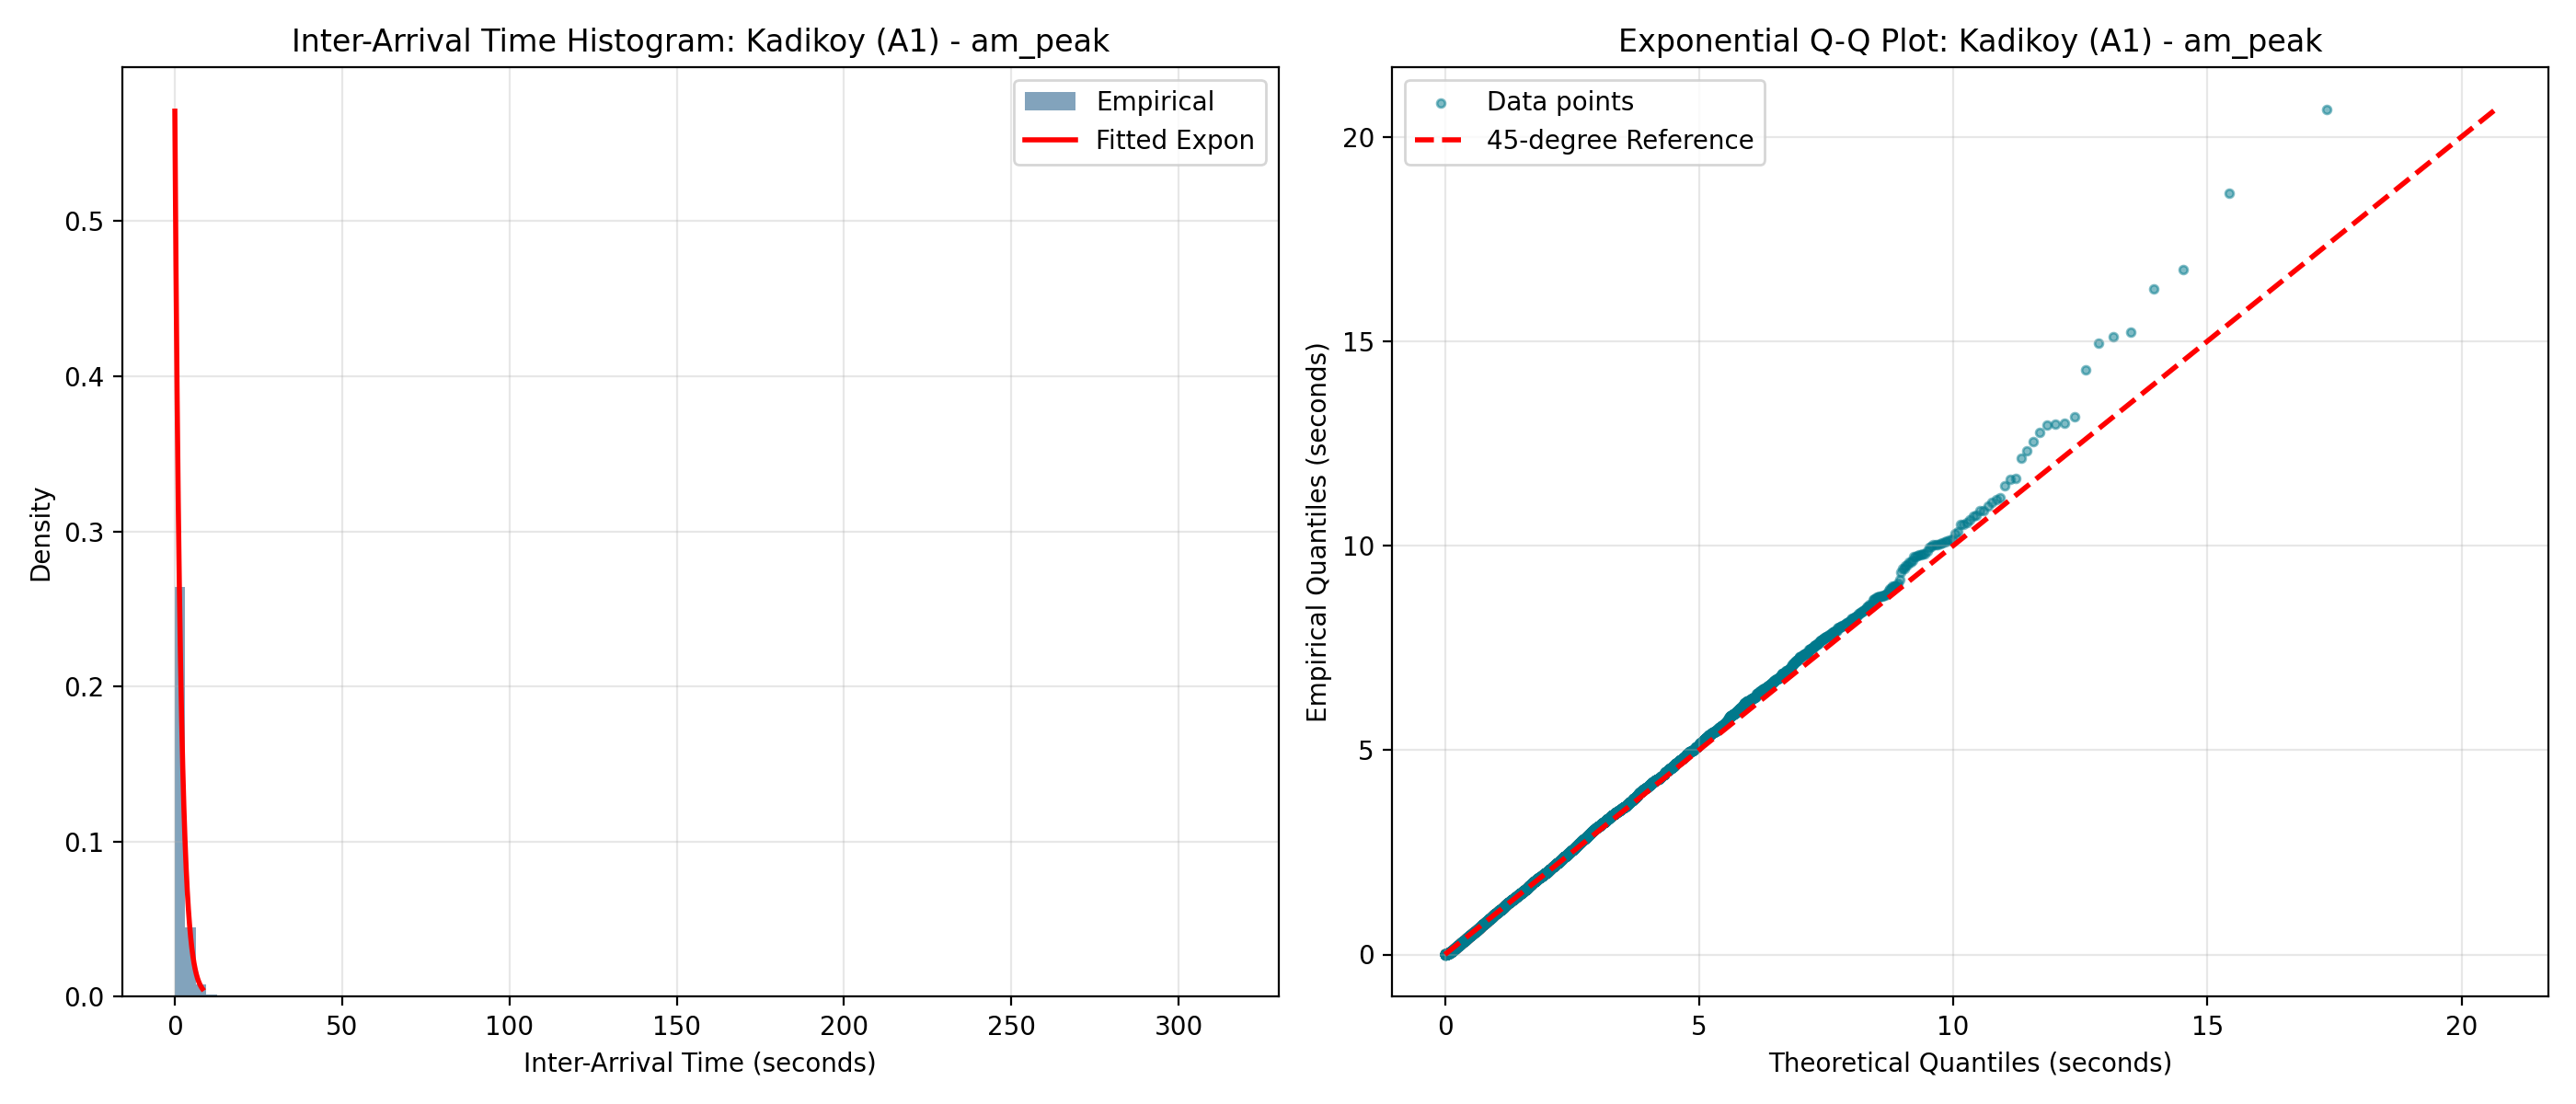
\includegraphics[width=0.47\textwidth]{plots/input_analysis/kadikoy_a1_am_peak_fit.png}
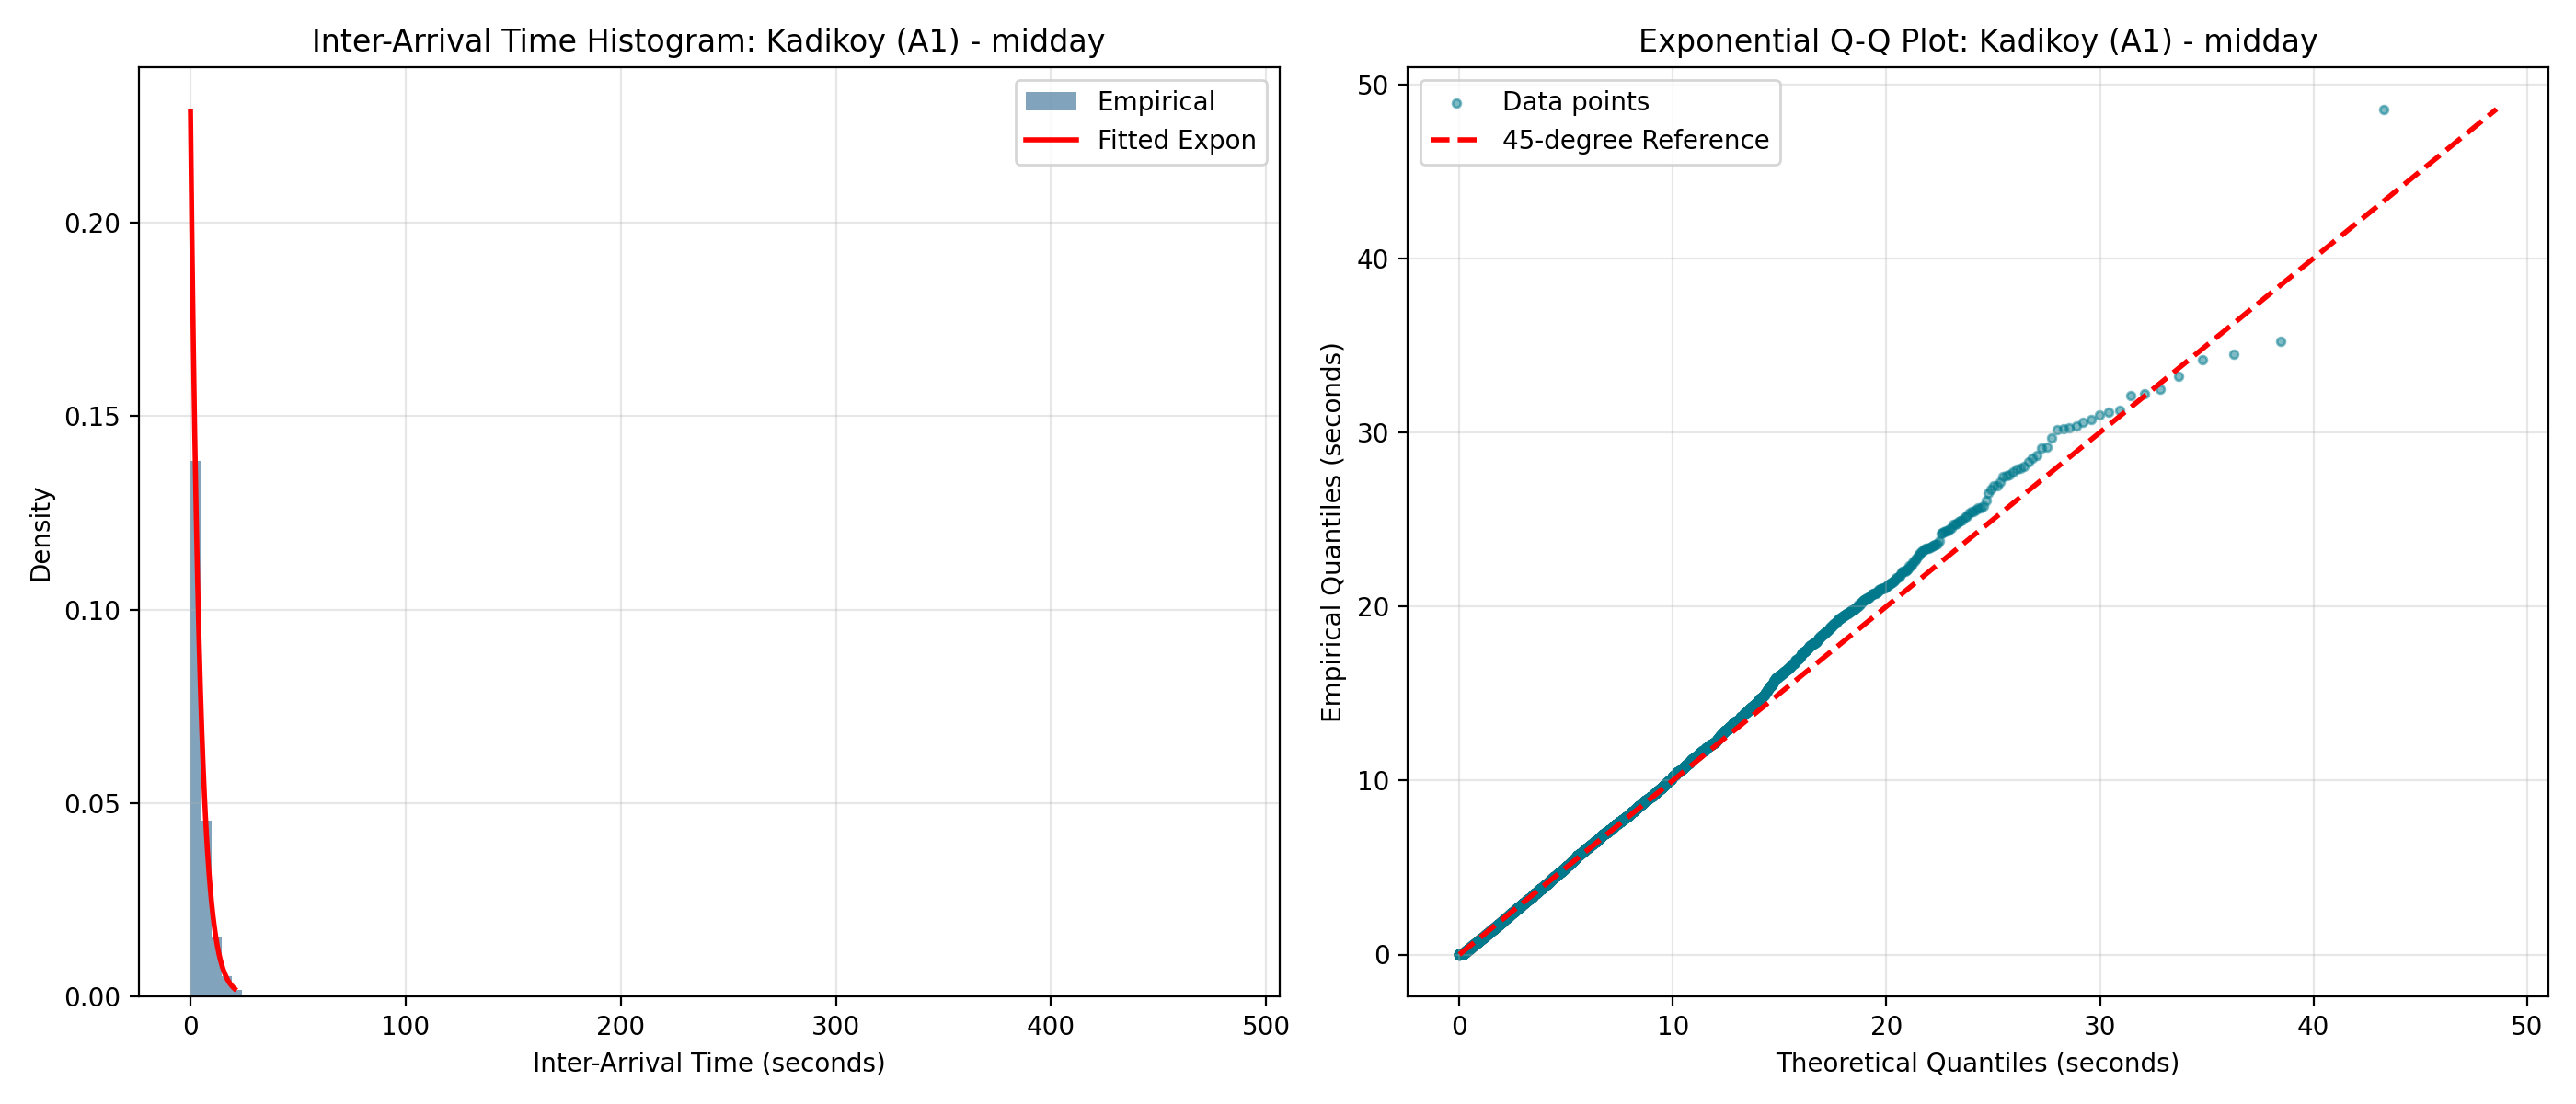
\includegraphics[width=0.47\textwidth]{plots/input_analysis/kadikoy_a1_midday_fit.png}
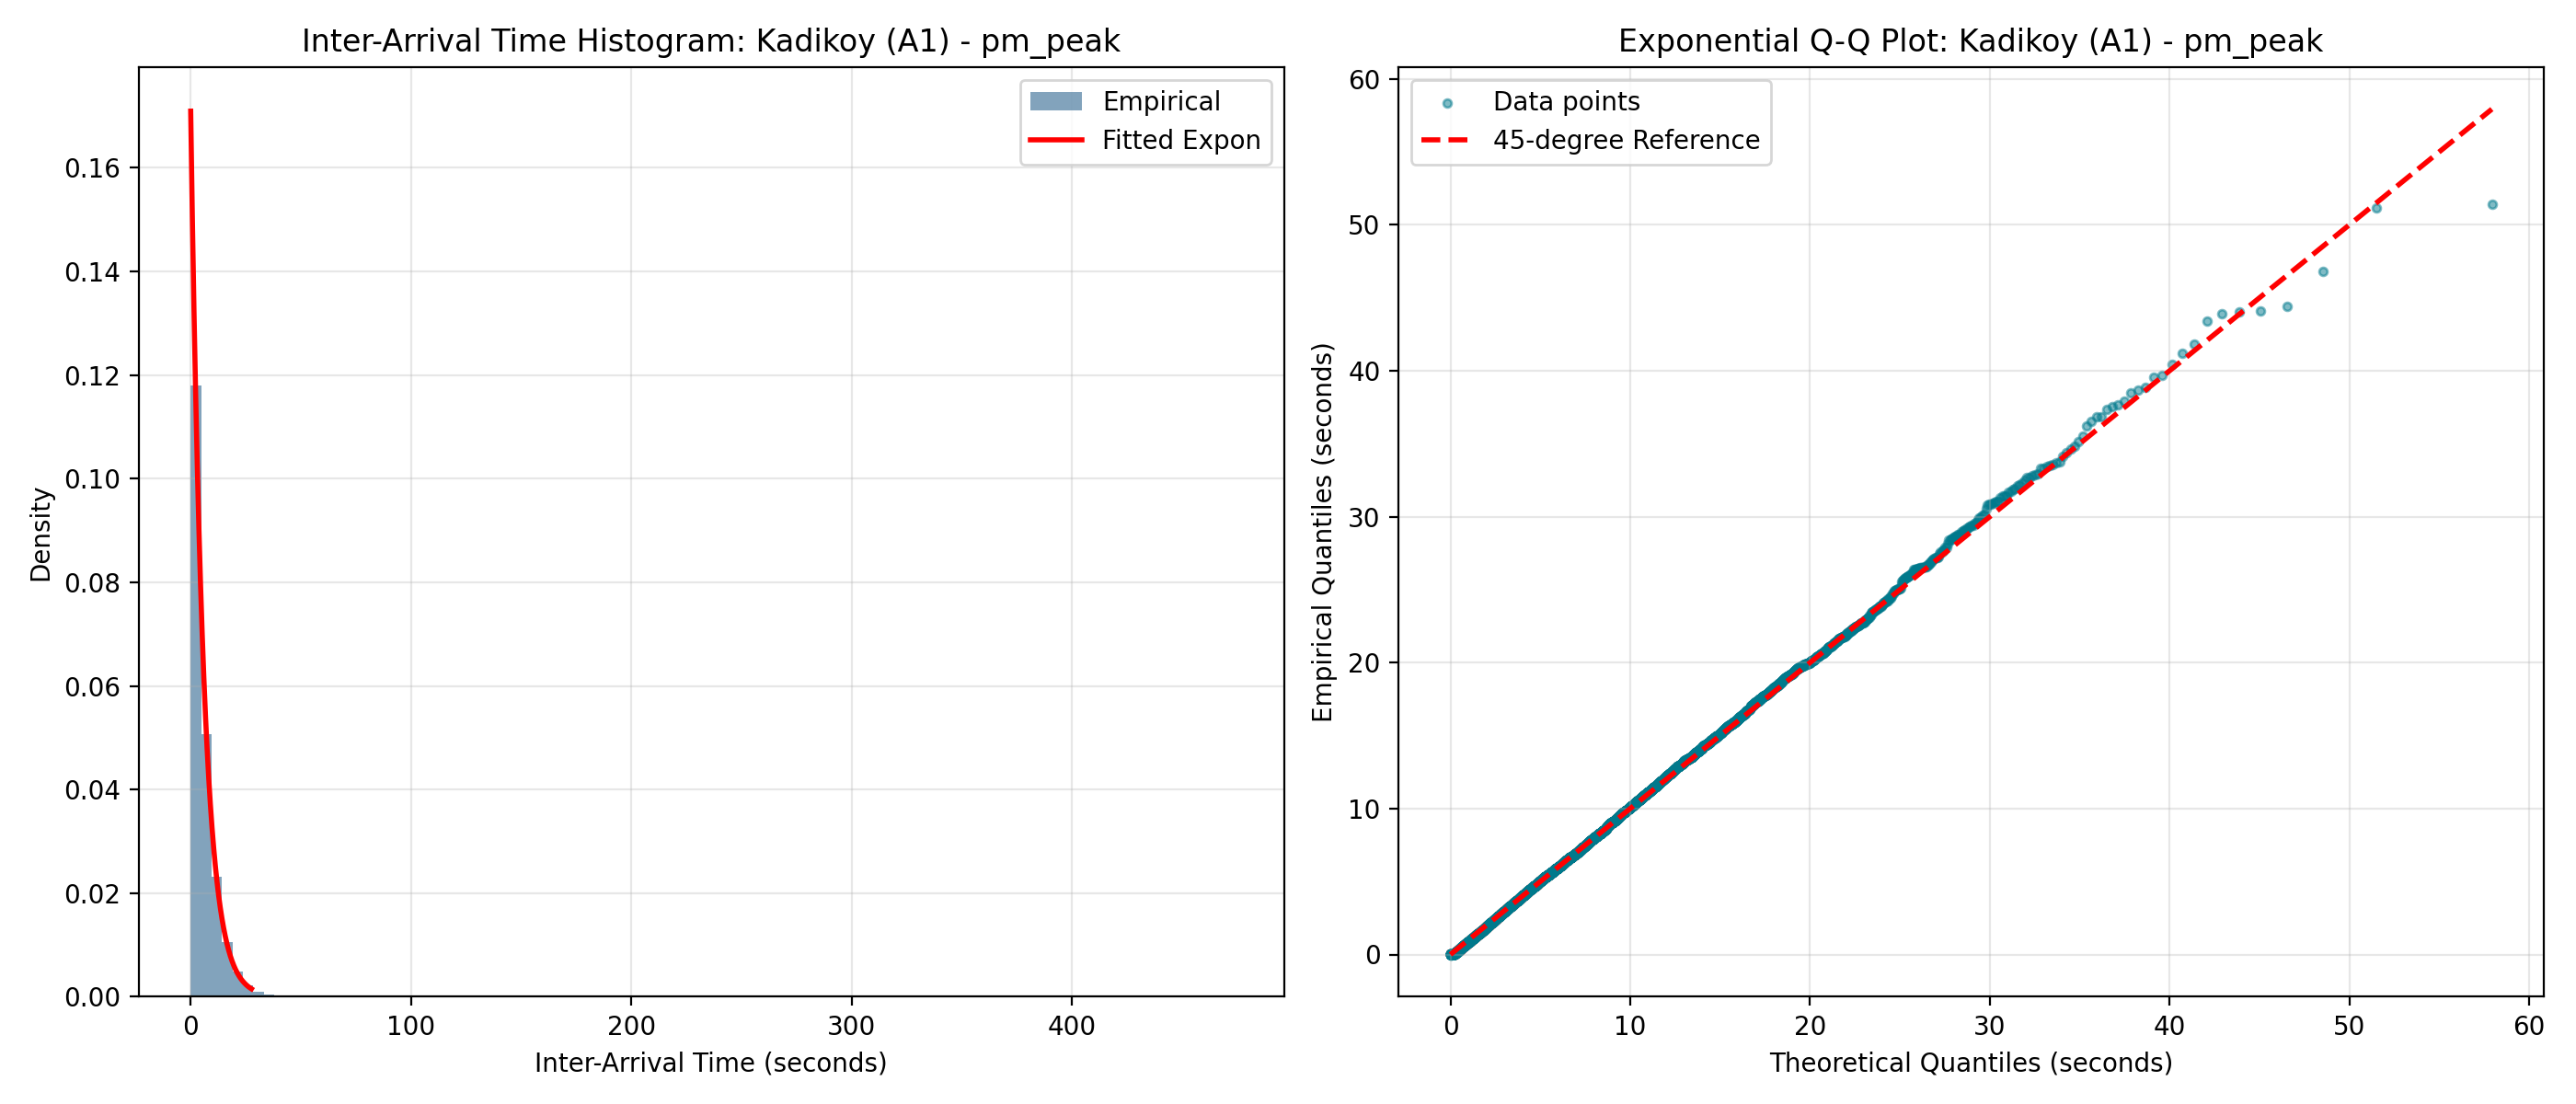
\includegraphics[width=0.47\textwidth]{plots/input_analysis/kadikoy_a1_pm_peak_fit.png}
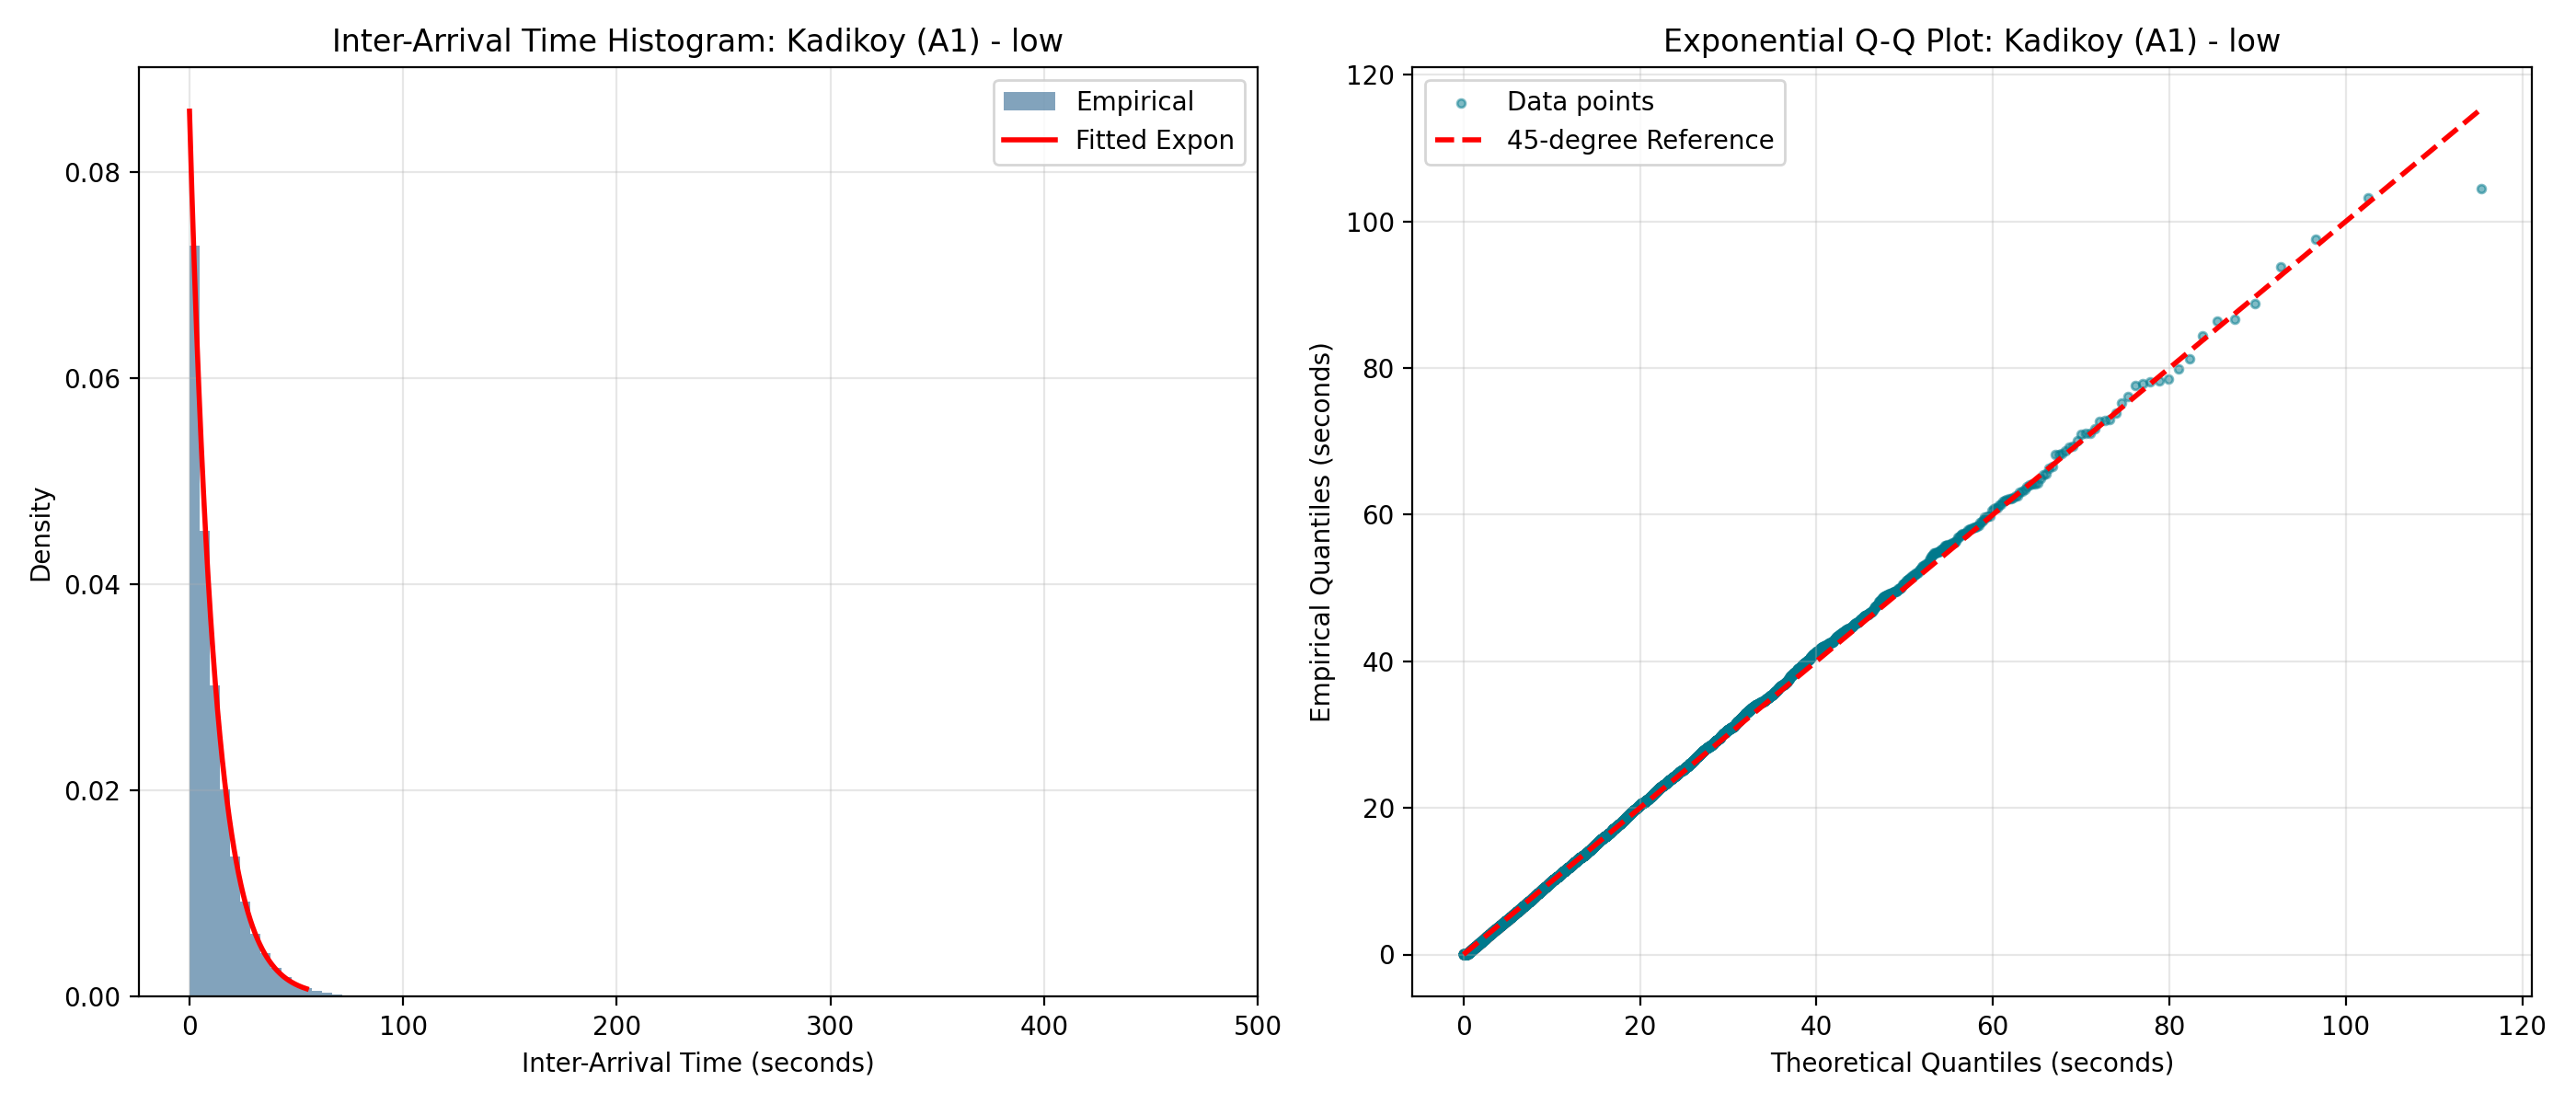
\includegraphics[width=0.47\textwidth]{plots/input_analysis/kadikoy_a1_low_fit.png}
\caption{Kad\i k\"{o}y fitted exponential histograms and Q-Q plots by period.}
\label{fig:kadikoy_plots}
\end{figure}

\begin{figure}[H]
\centering
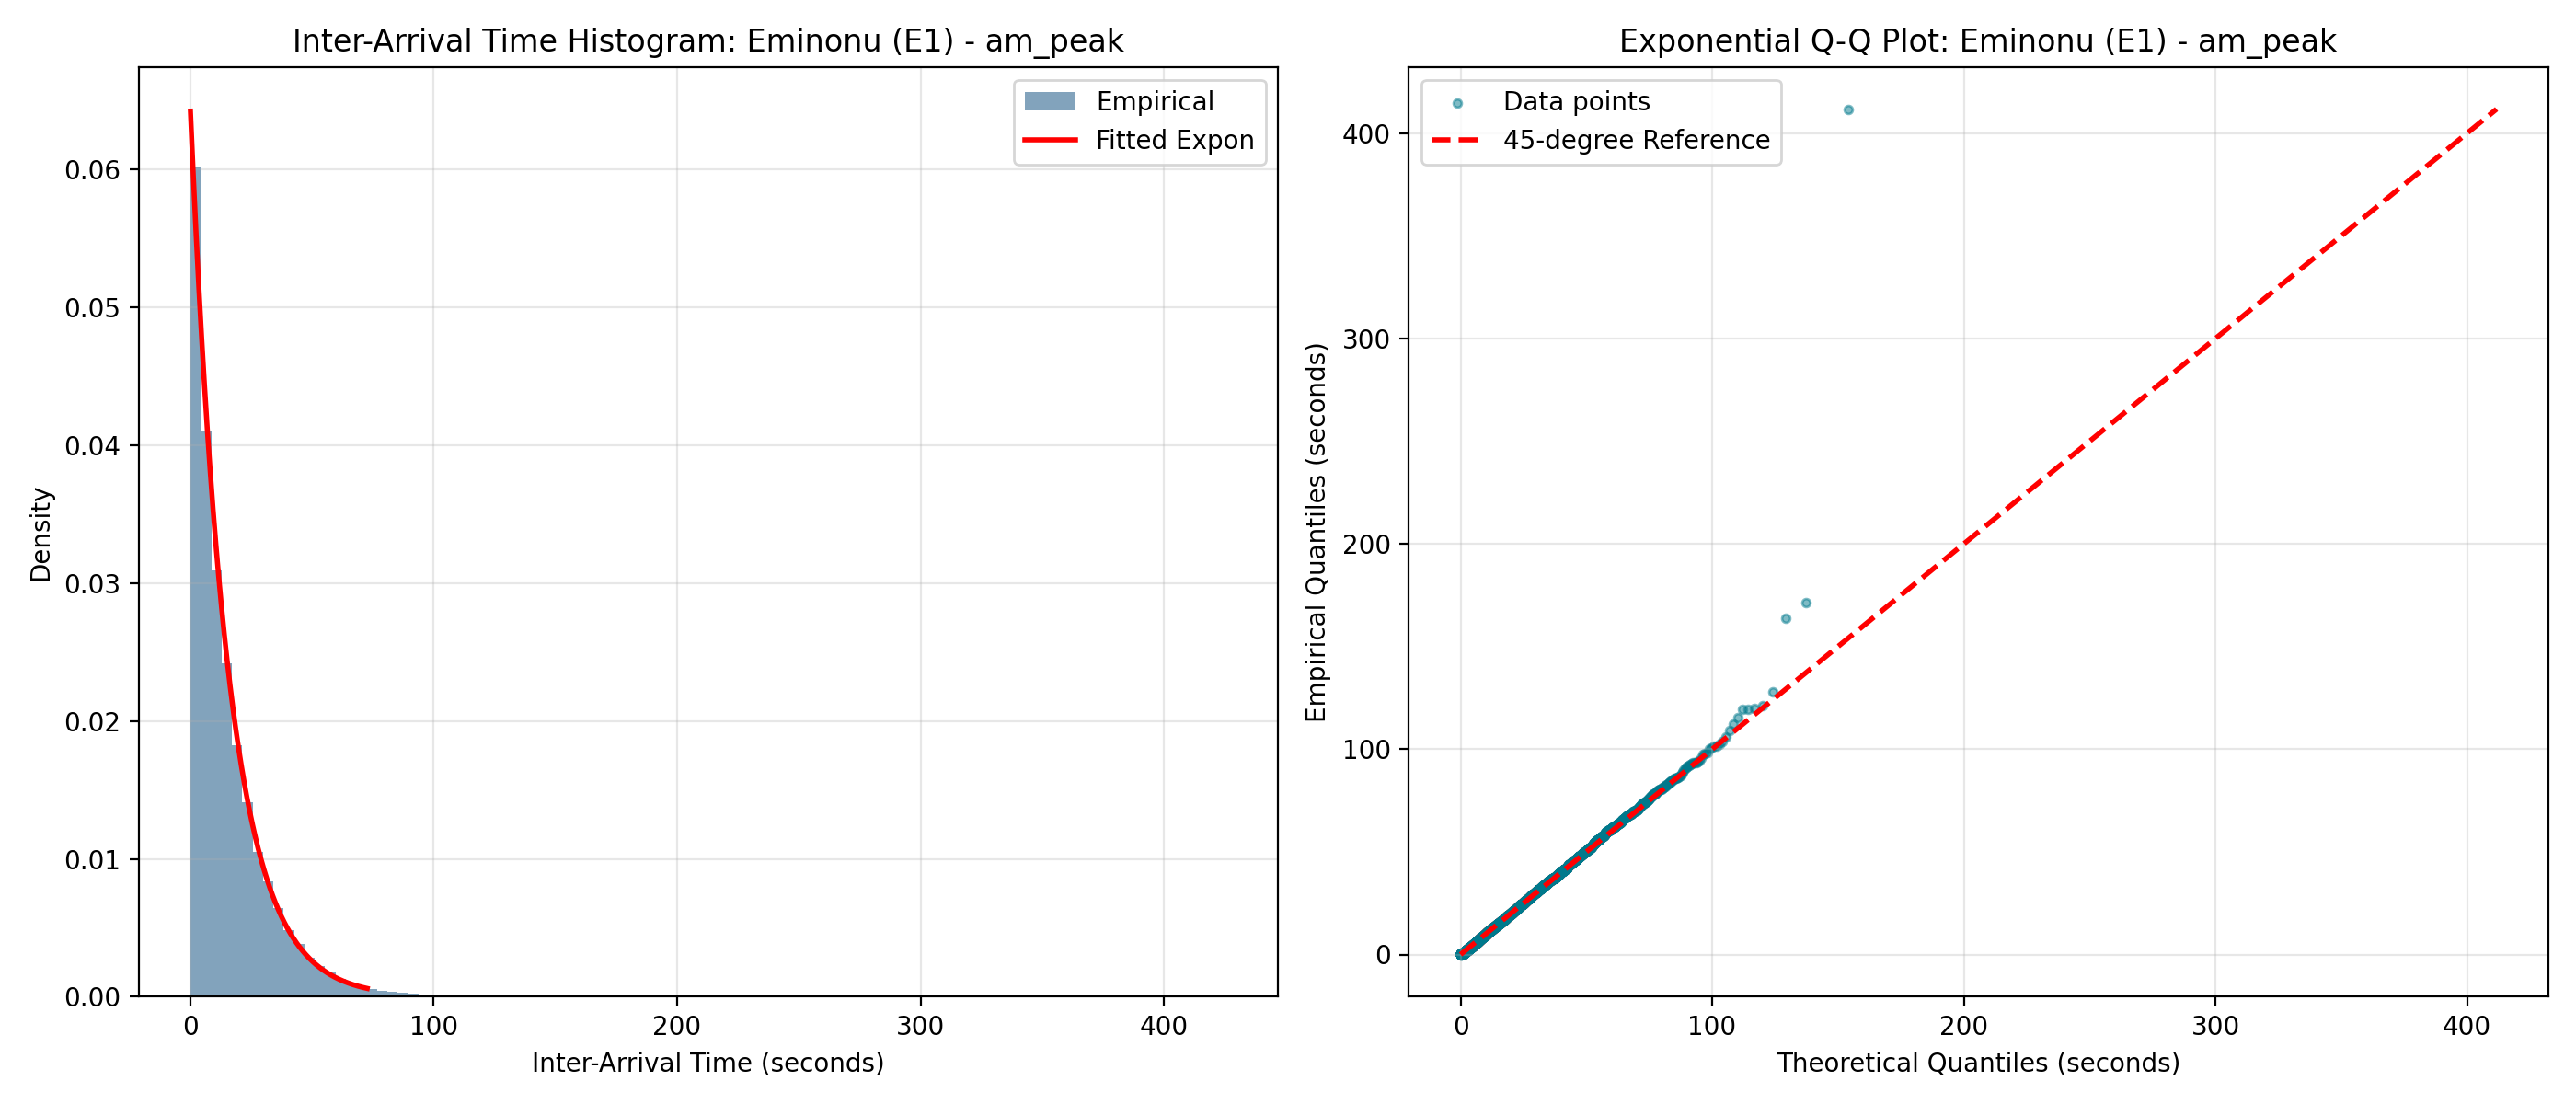
\includegraphics[width=0.47\textwidth]{plots/input_analysis/eminonu_e1_am_peak_fit.png}
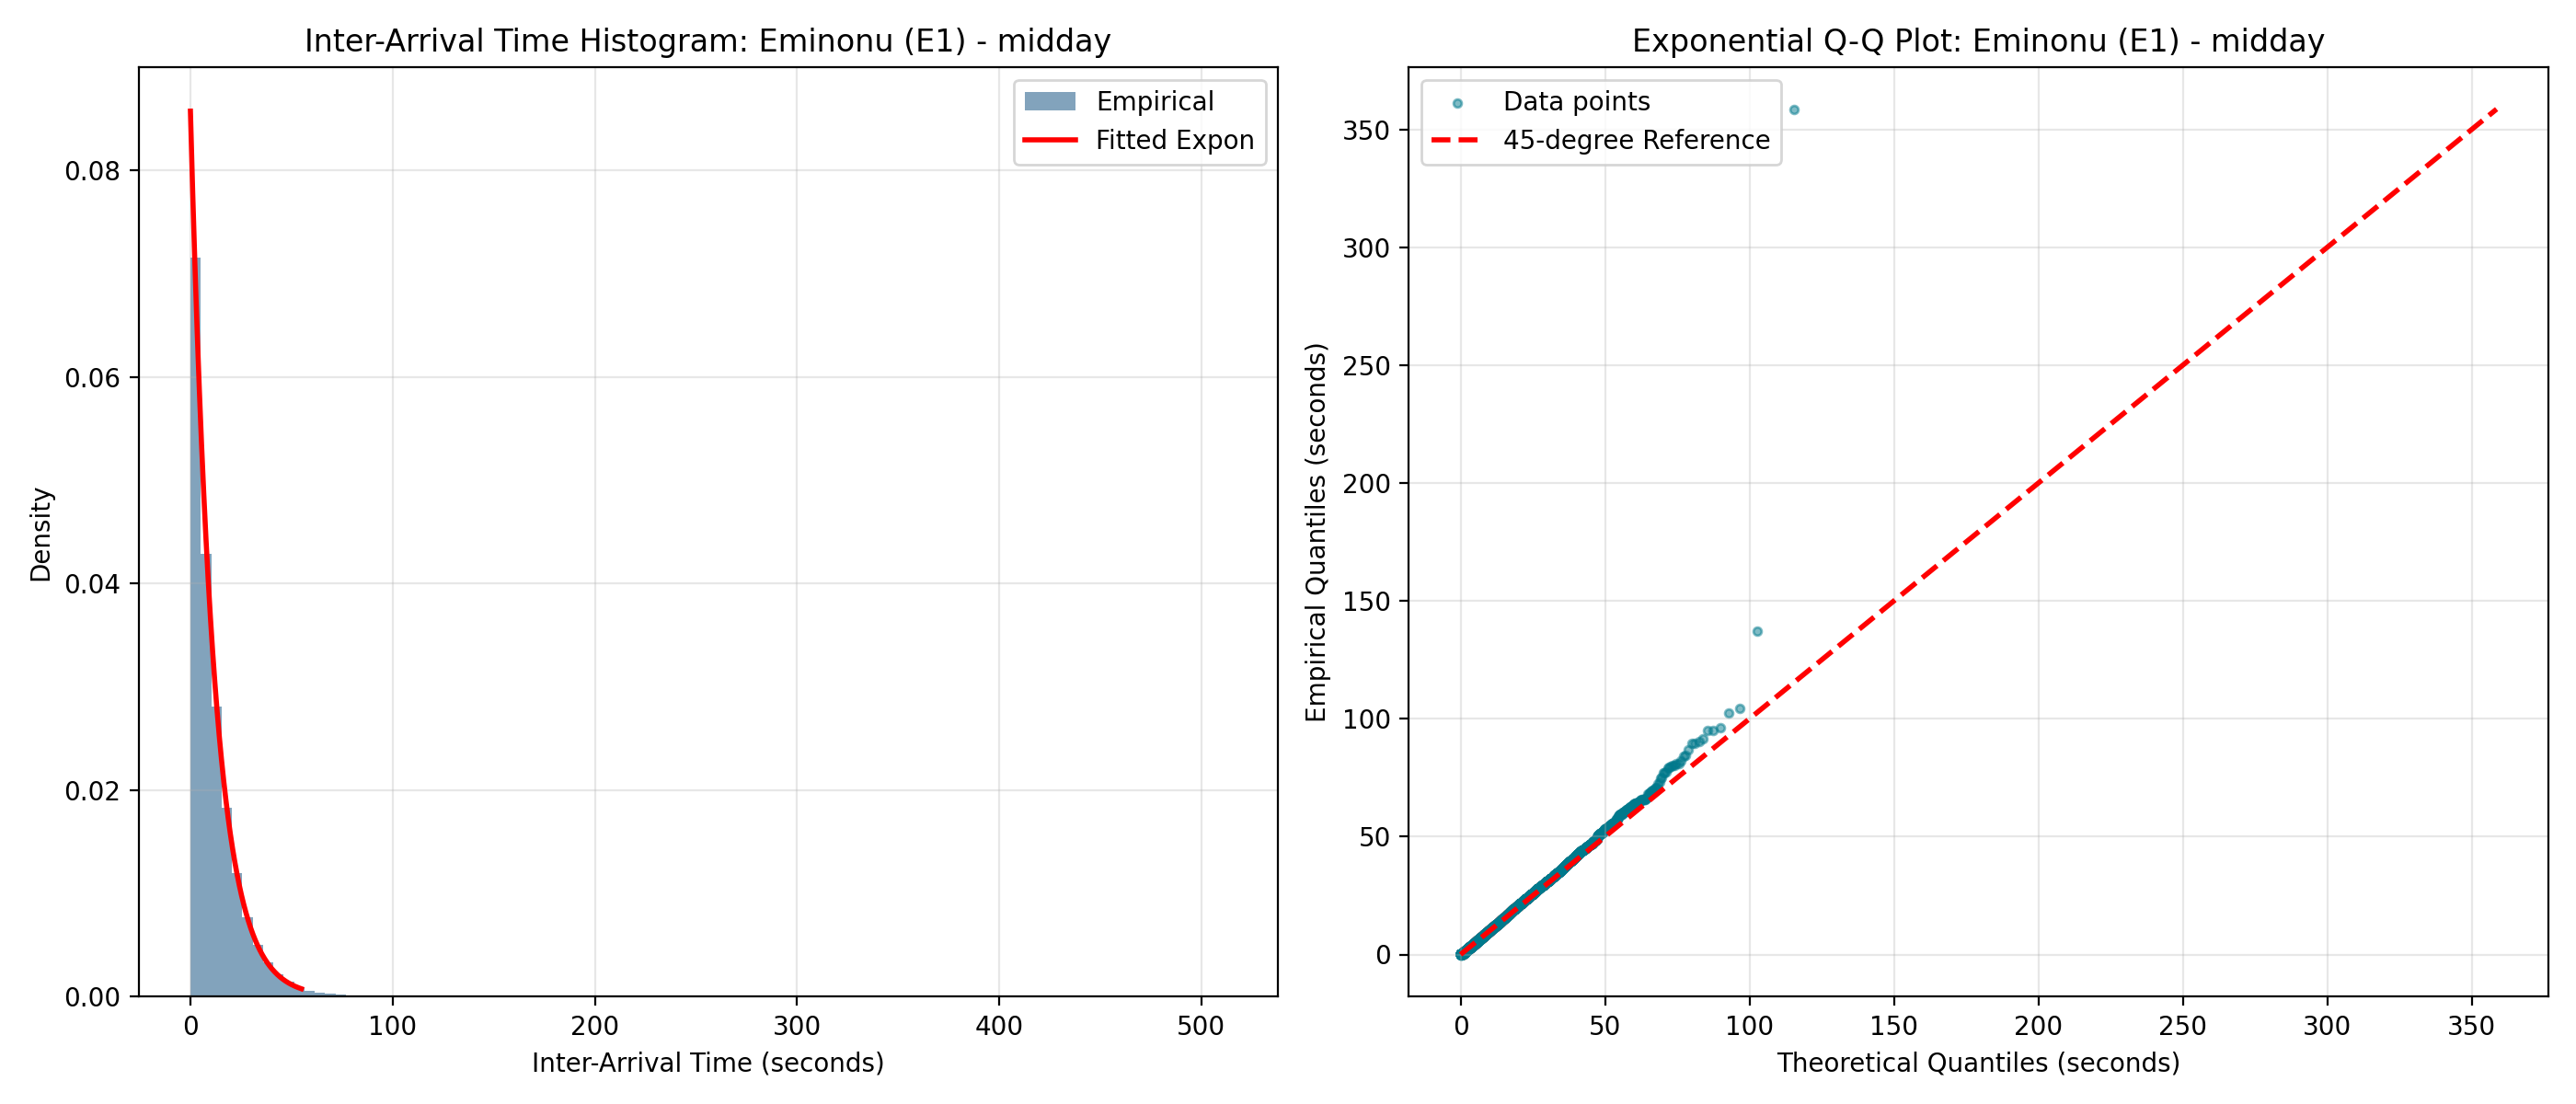
\includegraphics[width=0.47\textwidth]{plots/input_analysis/eminonu_e1_midday_fit.png}
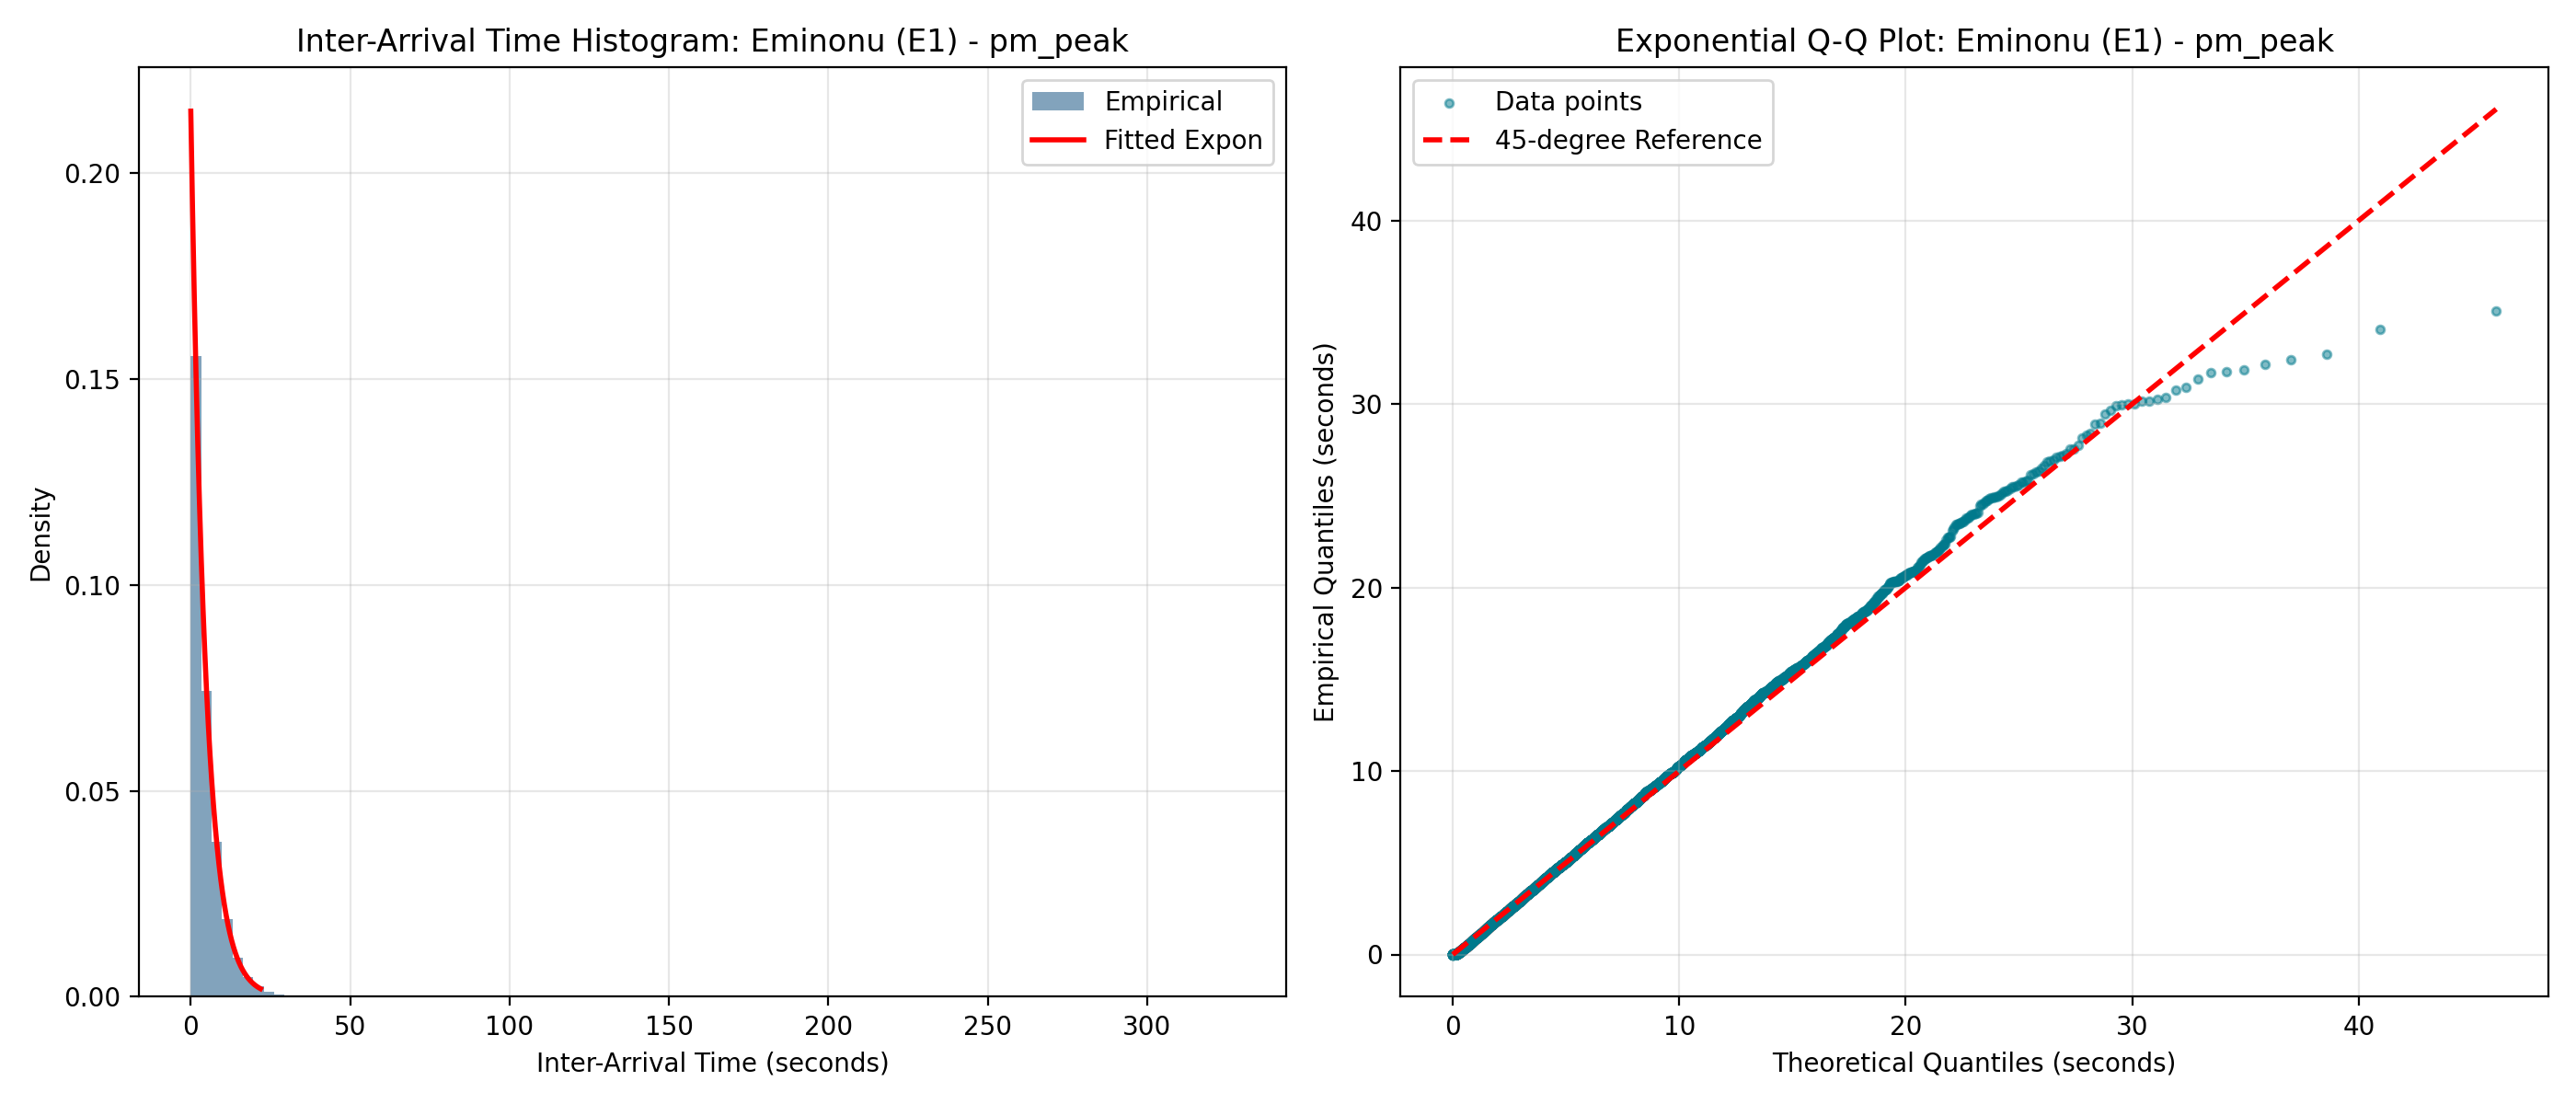
\includegraphics[width=0.47\textwidth]{plots/input_analysis/eminonu_e1_pm_peak_fit.png}
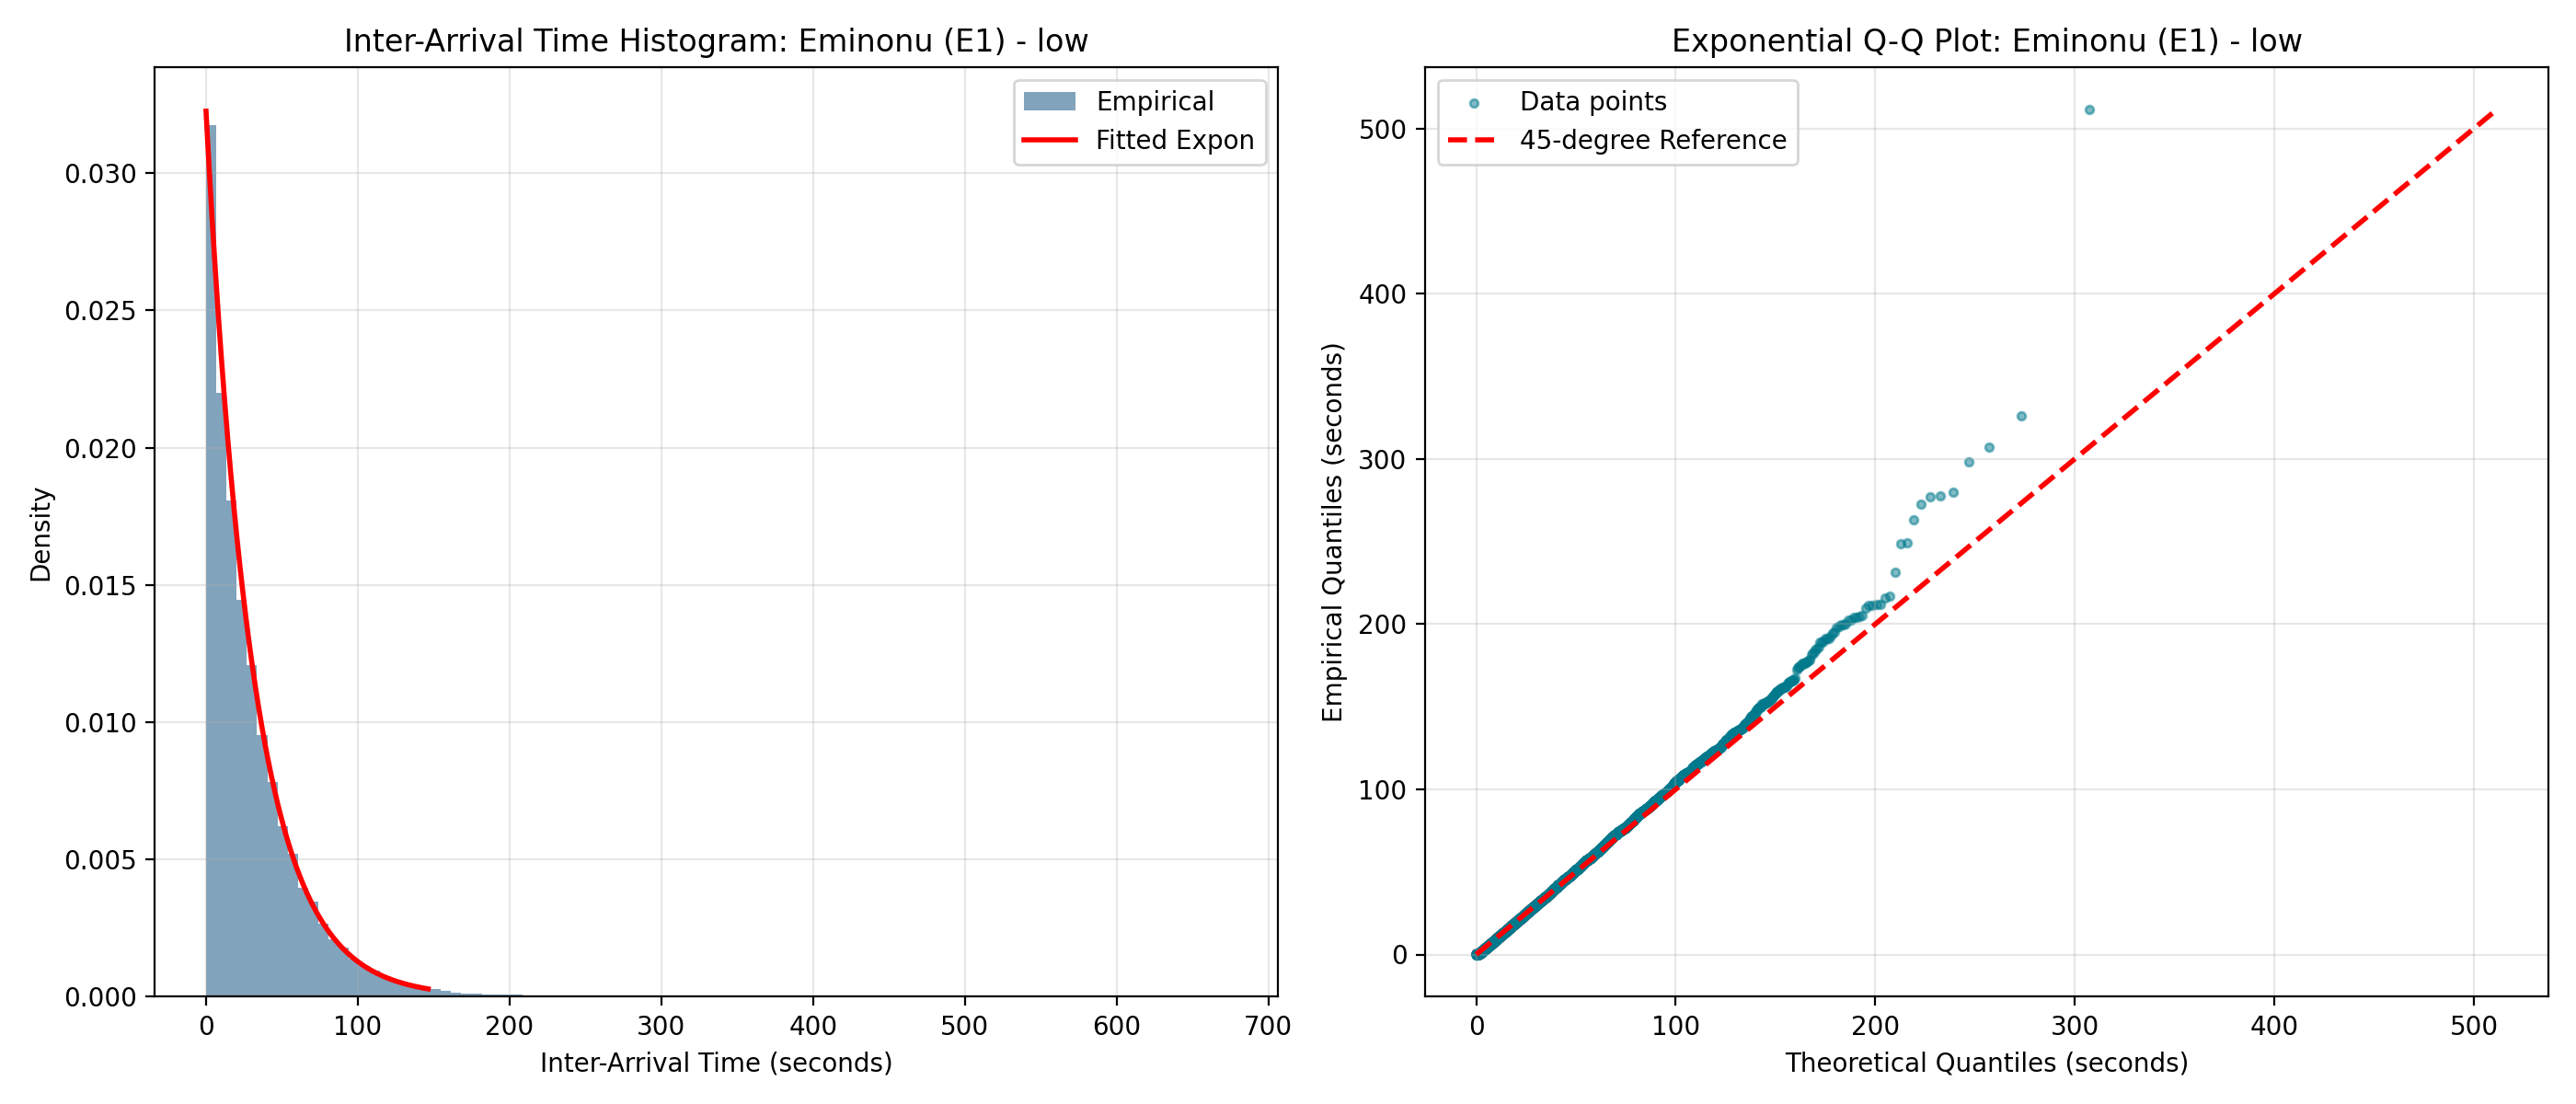
\includegraphics[width=0.47\textwidth]{plots/input_analysis/eminonu_e1_low_fit.png}
\caption{Emin\"{o}n\"{u} fitted exponential histograms and Q-Q plots by period.}
\label{fig:eminonu_plots}
\end{figure}

\section{Experimental Design}
The model uses separate NumPy \code{default_rng()} streams for arrivals, destination assignment, turnstile service, boarding service, route switching, and weather by directed line. Each replication uses the same base seed across scenarios, so the arrival sequences and passenger-level attributes are synchronized for common random numbers. The simulation window is 06:00--22:00; KPIs exclude passengers arriving before 07:00 and passengers not completed by 22:00.

\begin{table}[H]
\centering
\caption{Scenarios}
\label{tab:scenarios}
\begin{tabular}{lccc}
\toprule
\textbf{Scenario} & \textbf{Frequency} & \textbf{Shuttle} & \textbf{Weather} \\
\midrule
S1 Baseline & Standard & No & Calm \\
S2 High frequency & Headways $\times 2/3$ & No & Calm \\
S3 Shuttle network & Standard & Yes & Calm \\
S4 Storm stress test & Standard & No & Lodos, $p=0.20$ \\
S5 Full intervention & Headways $\times 2/3$ & Yes & Lodos, $p=0.20$ \\
S6 Custom intermediate capacity & Headways $\times 0.8$ & No & Calm \\
\bottomrule
\end{tabular}
\end{table}

\section{Results}
Table \ref{tab:simulation_results} reports means and 95\% t-confidence intervals over 20 replications. The required CSV files keep all time KPIs in seconds; this table converts time values to minutes for readability.

\begin{table}[H]
\centering
\caption{Simulation performance metrics (mean and 95\% confidence interval)}
\label{tab:simulation_results}
\resizebox{\textwidth}{!}{
\begin{tabular}{lcccccc}
\toprule
\textbf{Metric} & \textbf{S1} & \textbf{S2} & \textbf{S3} & \textbf{S4} & \textbf{S5} & \textbf{S6} \\
\midrule
\code{avg_journey_time} (min) & 40.27 [39.88, 40.67] & 30.54 [30.51, 30.56] & 36.49 [36.43, 36.55] & 66.96 [64.24, 69.69] & 37.55 [36.80, 38.29] & 32.81 [32.78, 32.83] \\
\code{avg_wait_kadikoy} (min) & 17.89 [17.09, 18.69] & 4.74 [4.70, 4.78] & 10.23 [10.13, 10.34] & 53.88 [48.55, 59.20] & 10.71 [9.73, 11.69] & 6.59 [6.54, 6.64] \\
\code{avg_wait_uskudar} (min) & 18.51 [17.90, 19.12] & 9.20 [9.15, 9.26] & 16.30 [16.18, 16.42] & 52.77 [45.26, 60.27] & 19.93 [17.73, 22.13] & 11.99 [11.94, 12.04] \\
\code{avg_wait_eminonu} (min) & 8.46 [8.41, 8.51] & 4.29 [4.25, 4.33] & 8.24 [8.19, 8.29] & 15.74 [14.42, 17.06] & 8.52 [7.93, 9.10] & 6.02 [5.97, 6.07] \\
\code{avg_wait_besiktas} (min) & 14.74 [14.62, 14.86] & 8.56 [8.45, 8.66] & 14.72 [14.60, 14.84] & 25.57 [23.85, 27.29] & 14.70 [13.85, 15.56] & 11.46 [11.40, 11.53] \\
\midrule
\code{loss_rate} & 0.000 & 0.000 & 0.000 & 0.035 [0.025, 0.045] & 0.001 [0.000, 0.001] & 0.000 \\
\code{left_behind_rate} & 0.123 [0.116, 0.130] & 0.002 [0.001, 0.002] & 0.030 [0.028, 0.033] & 0.331 [0.306, 0.357] & 0.074 [0.060, 0.088] & 0.003 [0.002, 0.004] \\
\code{missed_conn_rate} & 0.000 & 0.000 & 0.001 [0.000, 0.003] & 0.000 & 0.237 [0.152, 0.322] & 0.000 \\
\midrule
\code{load_factor_L1} & 0.376 & 0.251 & 0.384 & 0.465 & 0.324 & 0.298 \\
\code{load_factor_L2} & 0.555 & 0.378 & 0.534 & 0.675 & 0.452 & 0.456 \\
\code{load_factor_L3} & 0.444 & 0.302 & 0.450 & 0.529 & 0.396 & 0.365 \\
\code{load_factor_L4} & 0.534 & 0.350 & 0.524 & 0.628 & 0.420 & 0.435 \\
\midrule
\code{berth_util_kadikoy} & 0.149 & 0.220 & 0.149 & 0.121 & 0.176 & 0.184 \\
\code{berth_util_eminonu} & 0.149 & 0.220 & 0.282 & 0.116 & 0.335 & 0.184 \\
\code{throughput} (pax/hr) & 1774.6 & 1778.1 & 1774.6 & 1699.8 & 1772.1 & 1782.9 \\
\code{total_pax_served} & 26619.2 & 26671.9 & 26619.2 & 25497.6 & 26581.2 & 26742.9 \\
\bottomrule
\end{tabular}
}
\end{table}

Frequency is the strongest calm-weather lever: S2 lowers average journey time by 24.2\% and nearly eliminates left-behind events. S6 captures much of that benefit with fewer added sailings, so it is the more efficient calm-weather recommendation. The shuttle alone reduces left-behind rate from 12.3\% to 3.0\%, but it cannot match the direct capacity effect of higher frequency. Lodos primarily damages left-behind and loss-rate KPIs: S4 raises average journey time to 66.96 minutes, creates a 33.1\% left-behind rate, and causes 3.51\% balking. S5 restores storm performance close to calm baseline, though shuttle transfer reliability deteriorates because L5 departures can also be cancelled.

\section{Sensitivity Analysis}
We varied two storm-condition factors around S4 while keeping the standard network and no shuttle: cancellation probability and waiting-area capacity. Table \ref{tab:sensitivity} reports selected means and confidence intervals. Time is again shown in minutes.

\begin{table}[H]
\centering
\caption{Sensitivity analysis around S4 storm conditions}
\label{tab:sensitivity}
\begin{tabular}{lcccc}
\toprule
\textbf{Variant} & \textbf{Avg journey (min)} & \textbf{Loss rate} & \textbf{Left-behind rate} & \textbf{Throughput} \\
\midrule
$p_{\text{cancel}}=0.10$ & 52.14 [50.38, 53.91] & 0.004 & 0.238 & 1764.3 \\
$p_{\text{cancel}}=0.20$ & 66.96 [64.24, 69.69] & 0.035 & 0.331 & 1699.8 \\
$p_{\text{cancel}}=0.30$ & 80.04 [77.85, 82.23] & 0.084 & 0.385 & 1597.0 \\
Capacity $\times 0.75$ & 61.02 [59.30, 62.73] & 0.059 & 0.272 & 1659.2 \\
Capacity $\times 1.25$ & 70.60 [66.89, 74.30] & 0.021 & 0.364 & 1720.0 \\
\bottomrule
\end{tabular}
\end{table}

Cancellation probability has the largest system-wide impact: increasing $p_{\text{cancel}}$ from 0.10 to 0.30 adds 27.9 minutes to average journey time and reduces throughput by 167 pax/hr. Waiting capacity mainly changes whether excess demand is lost or retained. Increasing capacity reduces balking but can increase measured journey time and left-behind rate because more passengers remain in the congested system instead of leaving.

\section{Verification and Validation}
We performed the following checks before finalizing the outputs.
\begin{itemize}
    \item \textbf{Format and CI verification}: \code{results.csv} contains 2400 rows (6 scenarios $\times$ 20 replications $\times$ 20 KPIs), and \code{summary.csv} contains 120 rows. Recomputed t-intervals matched every \code{summary.csv} row exactly within floating-point tolerance.
    \item \textbf{CRN check}: For each replication, S1 and S2 \code{total_pax_served} differed by at most 0.257\%, well within the 2\% CRN check described in the rubric.
    \item \textbf{Headway check}: The 50\% frequency rule rounds baseline headways as required: 15$\rightarrow$10, 20$\rightarrow$13, 30$\rightarrow$20, 40$\rightarrow$27, and 60$\rightarrow$40 minutes.
    \item \textbf{Directional sanity checks}: S2 average journey time is below S1 (30.54 vs. 40.27 min); S4 loss rate exceeds S1 (3.51\% vs. 0); S5 loss rate is below S4 (0.065\% vs. 3.51\%); and S3 left-behind rate is below S1 (3.0\% vs. 12.3\%).
    \item \textbf{Deterministic smoke test}: A single manually injected A1$\rightarrow$E1 passenger boards, arrives, and is not marked balked, confirming the direct-routing and event lifecycle path.
\end{itemize}

\section{Conclusions}
For normal operations, S6 is the recommended steady policy because it gives a large journey-time reduction without the larger operating burden of S2. For Lodos warnings, the model supports activating S5: higher frequencies plus L5 restore throughput and nearly eliminate balking. The sensitivity analysis shows that cancellation probability is the dominant storm-risk driver, so accurate weather-triggered operating policy matters more than simply expanding terminal waiting capacity.

\end{document}
